\documentclass{article}
\usepackage{hyperref}
\usepackage{tabularx}
\usepackage{float}
\usepackage[export]{adjustbox}
\usepackage{titlesec}

\titleformat{\section}
{\Large\bfseries}
{}
{0em}
{}

\titleformat{\subsection}
{\large\bfseries}
{}
{0em}
{}

\begin{document}

\begin{figure}
    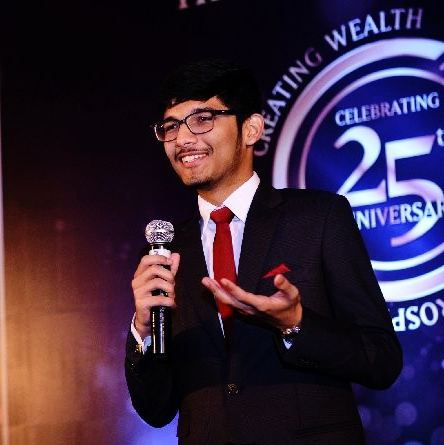
\includegraphics[width=.3\textwidth,right]{download}
    % \caption{right aligned image}
\end{figure}

\title{Aniruddha Chauhan}
\maketitle

\section{Contact Information}
A-2 Block \\  Paschim Vihar \\ New Delhi-110063
\\Contact: +91-95600 46060
\\ Email: \href{mailto:aniruddhac7@gmail.com}{aniruddhac7@gmail.com} 
				\and  \href{mailto:mail@aniruddhachauhan.com}{, mail@aniruddhachauhan.com}
\\ LinkedIn: \href{https://www.linkedin.com/in/anni-511/}{linkedin.com/in/anni-511/}
\\ Website: \href{http://www.aniruddhachauhan.com/}{aniruddhachauhan.com/}

\section{Career Objective}
I am a diligent worker with a knack for problem-solving, I like treading on new paths and to take up daunting challenges. I have an inclination towards Data Science and Artificial Intelligence, I want to leverage my knowledge of these two disciplines in the field of Finance and NLP. I am passionate about solving problems in a research-based environment and want to work as a researcher in close collaboration with Industry. 


\restylefloat{table}
\begin{table}
\begin{tabular}{|c|p{1.25in}|p{1in}|p{1in}|}
\hline
\textbf{Course/Examination} & \textbf{School/University} & \textbf{Year of Passing} & \textbf{Percentage}   \\ \hline
         B.Tech (CSE)&Bharati Vidyapeeth's College of Engineering, New Delhi&2020&71.39      \\
        CBSE Class 12  &Bal Bharati Public School, Pitampura, New Delhi      &      2016     &      94.4       \\ 
        CBSE Class 10  &     Bal Bharati Public School, Pitampura, New Delhi      &      2014     &      93.1 (9.8 CGPA)    \\	\hline
\end{tabular}
\end{table}

\section{Projects}
{\begin{enumerate}


\item \subsection{News Analytics Tool}
 This is an ongoing project where I'm bulding a media tool similar to MIT's Media Cloud but having more advanced functionalities like, Topic Modeling, Extracting Keywords, Bias Detection, Fake News Detection etc. 
\item \subsection{Pollinator Bee}
 This project involves mimicking the behaviour of a bee using a UAV in this project PlutoX was used, the drone has to hover over a flower which has an incomplete circuit that is completed when a conducive material attached to the drone comes in contact with the flower. The controlling of drone was done via ROS.
\item \subsection{Classification of Fake News by Fine-tuning Deep Bidirectional Transformers based Language Model}
  In this project, I use an NLP approach to classify fake news and real news, with the help of state-of-art BERT language model. The corpus we use contains only
the text present in the body of the news articles. After extensive experimentation, the model was
able to achieve an accuracy of 97.021\% .
\item \subsection{Chatbot using RASA Framework}
This project involves building a Chatbot using Django and RASA Framework, the Chatbot can be used to answer FAQs. This project involved end to end work, from data collection to preprocessing to making language models and then creating an API to send and recieve data using Django Framework. All the tasks were done in Python and HTML/CSS was also used.
\item \subsection{Property Stratification}
This project involved geo-plotting of Natural Hazards based on their severity. This is done to know which regions are prone to natural disasters, which is useful for Insurance Companies to adjust premiums while Insuring a property. I used Folium for plotting that used Leaflet.js and the data cleaning and preprocessing was done using Pandas and geoPandas. 


	
\end{enumerate}}



\section{Training and Internship}
\begin{itemize}
\item Research Project Intern at IIT-Delhi February 2019 - Present
\item Summer Decision Analytics Intern at EXL (Inductis) June 2018 - August 2018
\item Summer Intern at AAPNA Infotech July 2017 - August 2017
\end{itemize}

\section{Research Publications}
None yet, one paper is under review

\section{Technical Skills}
\begin{itemize}
\item Python
\item  Machine Learning and Deep Learning
\item C
\item C++
\item Java
\item  Pandas, Sklearn, Matplotlib, NLTK
\item  Django
\item  Folium
\item SQL
\item HTML, CSS, JavaScript
\item \LaTeX
\item PyTorch
\item Keras
\end{itemize}

\section{Soft Skills}

\begin{enumerate}
\item Proficiency in English and Hindi 
\item Ability to Work Under Pressure and Time Management
\item Effective Communication 
\item Can work with a Team and have good Leadership Qualities 
\end{enumerate}

\section{Co-Curricular Activities}

\begin{itemize}
\item Playing Football
\item Gaming 
\end{itemize}

\section{Co-Curricular Activities}

\begin{enumerate}
\item Winner of eYantra 2018 (Pollinator Bee)
\item Chairperson - BVPIEEE Computer Society (July 2018 - Present)
\item Research and Development Head - BVPIEEE Computer Society (August 2017 - June 2018)
\item Web Executive - ACM BVP (September 2016 - May 2017)
\end{enumerate}

\section{Personal Details}
Father's Name: Mr. Neeraj Chauhan
\\ Mother's Name: Mrs. Seema Chauhan
\\ Sex: Male
\\ Date of Birth: 5/11/1997
\\ Nationality: Indian
\\ Marital Status: Not Married

\section{Reference}
Mrs. Rituparna Datta (AVP EXL Email: \href{mailto:rituparna.datta@exlservice.com}{rituparna.datta@exlservice.com})
\\Mrs. Deepika Kumar (Assistant Professor Email: \href{mailto:deepika.kumar@bharatividyapeeth.edu}{deepika.kumar@bharatividyapeeth.edu})

\section{Declaration}
I hereby declare that the details mentioned above are accurate to the best of my knowledge.
\\Date: 17th April 2019
\end{document}